\chapter{Design}

\section{System Architecture}

As mentioned in section \ref{ch:reqandspec:sec:spec}, we have opted for a design that involves two applications. The main Rails on Rails app includes the grading library as one of its dependencies. In Ruby, adding a library as a dependency is the equivalent of adding the code of the library directly. That means that the main application can now call the library's code without any other requirement such as running the library independently.

\begin{figure}[H]
    \centering
    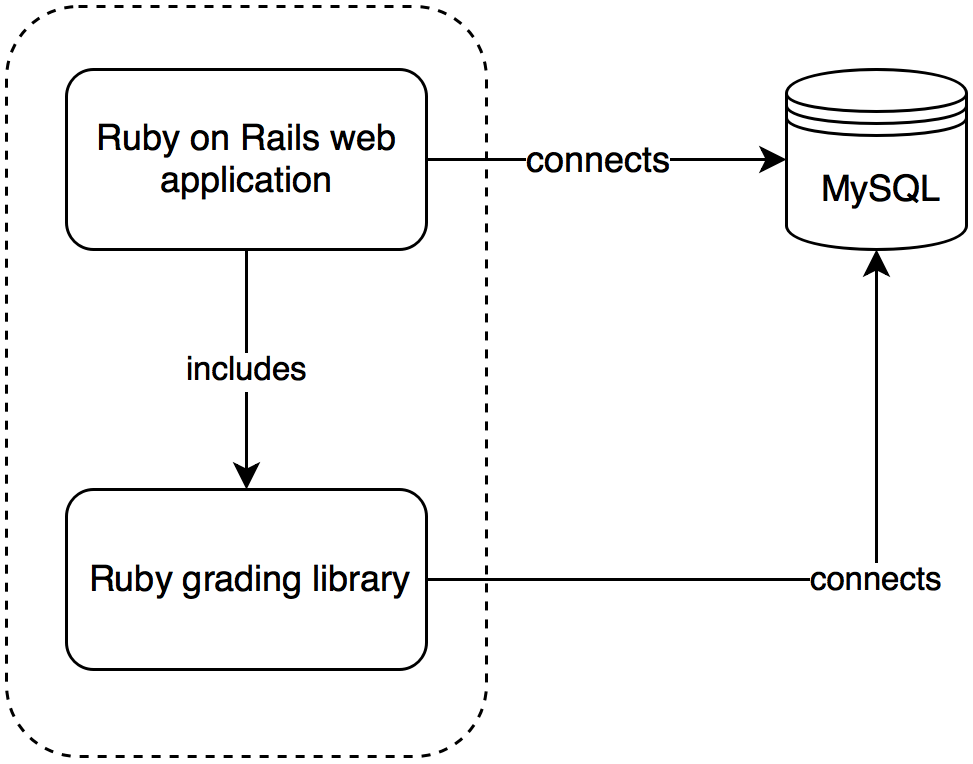
\includegraphics[width=(\linewidth / 2)]{Chapters/4-Design/sysarh.png}
    \caption{System architecture}
\end{figure}

Both the web application and will share the same MySQL server. However, they will both use different databases. A more in-depth explanation of how the library uses the database will be presented in section \ref{ch:impllib:sec:connecting}.

\section{Grading library}

The grading library is composed of multiple modular classes that have a single responsibility. The main entry point of the library is the \mintinline{ruby}{Assessor} class which is the public interface of the library. The library exposes two methods that are called by the main web application:

\begin{itemize}
    \item \mintinline[breaklines]{ruby}{def compile(create_schema_sql_query:, instructor_sql_query:, seed_sql_query:)} which is called by the web application when an exercise is returned. The method checks if the SQL queries submitted by the teacher are correct and if yes, what's the structure of the database.
    \item \mintinline[breaklines]{ruby}{def assess(create_schema_sql_query:, instructor_sql_query:, seed_sql_query:, student_sql_query:)} which returns the results of comparing a student's query with the instructor's query.
\end{itemize}

The library does not store any compilation results, or submission grades. Therefore, the results returned by these two methods must be saved by the caller if they want them to be stored permanently.

\subsection{Code structure}

One of the goals of the project is to build an application that can be easily extended in the feature. To do this, the library is split in many classes that each handle a very specific feature.

\begin{enumerate}
    \item The \mintinline{ruby}{Assessor} which exposes the public interface of the library and integrates all the other components of the library.
    \item \mintinline{ruby}{DatabaseConnection} which handles connecting to a database and running single statement queries (queries formed of a single command) and multi statement queries (queries formed of multiple commands). In addition, this class also implements the required security measures for running user's SQL.
    \item \mintinline{ruby}{DataExtractor} class looks over the extraction of data and schema of a database. This is used in the \mintinline[breaklines]{ruby}{compile()} method for returning the structure of the database.
    \item \mintinline{ruby}{QueryTransformer} class that handles the canonicalization process. This class sequentially (in a predefined order) runs transformers defined in the \mintinline{ruby}{Trasnformers::} namespace. Each class from the \mintinline{ruby}{Trasnformers::} namespace performs a single type of transformation. They take in a query, apply a set of transformations and then return the transformed query.
    \item \mintinline{ruby}{QueryAttributeExtractor} class which handles the extraction of various components of a query after a transformation has been made. In order to do that, it makes use of parsers defined in defined in the \mintinline{ruby}{Parsers::} namespace. Each class from the \mintinline{ruby}{Parsers::} namespace extracts a single attribute. Although we are using a parser to parse SQL, these classes allow us to remove unwanted syntax and to transformed the parsed elements to a format that suits us better.
    \item \mintinline{ruby}{QueryComparator} class which compares the results of two queries.
    \item \mintinline{ruby}{Graders::} namespace contains multiple graders whose job is to compare a single component of a query (e.g. \mintinline{ruby}{Graders::Columns} handles the assessment of the columns component)
    \item \mintinline{ruby}{QueryComparisonResult} class which represents the final result of the submission. It includes a grade, hint and grades of each component of the query. This class also calculated the partial grade based on the results of the QueryComparator, and a comparison between the actual components of the two SQL queries using the graders from \mintinline{ruby}{Graders::}
    \item In addition, the library also contains multiple \mintinline{ruby}{Error} classes that represent various errors that might happen during the execution of the process - such as the inability to establish a database connection (\mintinline{ruby}{DatabaseConnectionError})
\end{enumerate}

Splitting the functionality into multiple classes leads to cleaner code that allows faster development. In addition, this strategy makes use of encapsulation. For instance, no class other than \mintinline{ruby}{DatabaseConnection} knows how queries are exactly performed. The other classes simply know that \mintinline{ruby}{DatabaseConnection} provides a way to execute single and multi queries. This allowed the project to initially focus on the core aspect of it - the canonicalization process, before thinking about concurrency or security issues described in section \ref{ch:impllib:sec:connecting}.

\subsection{Compile method}
\begin{figure}[H]
\resizebox{\linewidth}{!}{
    \smartdiagramset{
        uniform sequence color=true,
        sequence item border color=black,
        sequence item text color=white,
        sequence item height=1.5cm
    }
    \smartdiagram[sequence diagram]{
        Create tables,
        Seed initial data,
        Execute correct query,
        Extract tables and data
    }
}
\caption{Overview of compile method}
\end{figure}

When compiling an assessment, a query will go through multiple steps:
\begin{tabularx}{\textwidth}{|c|Y|Y|}
    \hline
    \textbf{Step} & \textbf{Action} & \textbf{Code implementation} \\\hline
    \endhead
    1 & Acquire a database connection and handle any errors & Create a new \texttt{DatabaseConnection} and immediately return any potential \texttt{DatabaseConnectionError}. \\\hline
    2 & Create the database tables passed in the \texttt{create\_schema\_sql\_query} & Execute the \texttt{create\_schema\_sql\_query} on the \texttt{DatabaseConnection} and immediately return any potential \texttt{DatabaseSchemaError} \\\hline
    3 & Seed the database tables data provided by \texttt{seed\_sql\_query} & Execute the \texttt{seed\_sql\_query} on the \texttt{DatabaseConnection} and immediately return any potential \texttt{DatabaseSeedError} \\\hline
    4 & Try to execute the correct query to ensure that the instructor's query can actually be performed
    on the current database and that it does not contain any syntactic errors. & Execute the \texttt{instructor\_sql\_query} on the \texttt{DatabaseConnection} and immediately return any potential \texttt{DatabaseQueryExecutionFailed} \\\hline
    5 & Extract the tables and data from the database & Use \texttt{DataExtractor} to extract data and tables using the \texttt{DatabaseConnection}. \\\hline
\end{tabularx}

\subsection{Assess method}
\begin{figure}[h]
\resizebox{\linewidth}{!}{
    \smartdiagramset{
        uniform sequence color=true,
        sequence item border color=black,
        sequence item text color=white,
        sequence item height=2cm
    }
    \smartdiagram[sequence diagram]{
        Create initial tables and seed data,
        Execute the two queries,
        Canonicalize the queries,
        Extract the components of each query,
        Assign a grade based on components
    }
}
\caption{Overview of compile method}
\end{figure}

The assess method is fairly similar to the compile method. In fact, the steps 1-3 from compile method are also used in this method. The rest of the method continues as following:

\begin{tabularx}{\textwidth}{|c|Y|Y|}
    \hline
    \textbf{Step} & \textbf{Action} & \textbf{Code implementation} \\\hline
    \endhead
    4 & Execute and store the results of both the student's query and the instructor's query & Execute the \texttt{instructor\_sql\_query} and \texttt{student\_sql\_query} on the \texttt{DatabaseConnection} and return any potential \texttt{DatabaseQueryExecutionFailed} \\\hline
    5 & Compare the results obtained in step 4 & Execute \texttt{QueryComparator}'s compare method on the results of the two queries obtained in step 4. \\\hline
    6 & Canonicalize each query & Execute \texttt{QueryTransformer}'s transform method on each query. Internally, each query goes through multiple transformations performed by classes from \texttt{Transformers::} namespace. \\\hline
    7 & Extract the components of each query &  Execute \texttt{QueryAttributeExtractor}'s extract method on each query. Internally, each query component is obtained by multiple parsers performed by classes from \texttt{Parsers::} namespace. \\\hline
    8 & Compute the final grade and return the components, hints and grade to the caller &  Build a new \texttt{QueryComparisonResult}'s based on the result of the comparison of the results, and the components obtained in step 6. Internally, the partial grade is obtained by comparing each element. The comparison of each component is delegated to a class from \texttt{Graders::} namespace. Finally, assemble the final \texttt{QueryComparisonResult} which includes the full list of components, a hint based on the comparison, and the final grade\\\hline
\end{tabularx}


\begin{tabularx}{\textwidth}{|c|Y|Y|}

\end{tabularx}

\subsection{Canonicalization} \label{ch:lit:sec:improved_canon}

The library's canonicalization process will include all the transformations done by XData presented in section \ref{ch:lit:sec:canonicalization}. In addition to these, it also performs two more transformations:
\begin{enumerate}
    \item Transforming \mintinline{mysql}{*} in the full list of columns. This will ensure that the algorithm will not penalize students who type the full list of columns, instead of just using  \mintinline{mysql}{*}.
    \item Making MySQL default attributes explicit. For instance, every MySQL \mintinline{mysql}{SELECT} query has a default uniqueness filter of \mintinline{mysql}{ALL}. That means that, while explicitly mentioning \mintinline{mysql}{ALL} will have no effect, it will not make the query wrong either.
\end{enumerate}

The order in which transformations are performed is essential. For instance, the transformation of the BETWEEN predicate must happen before the transformation of \mintinline{mysql}{>=} to \mintinline{mysql}{<=}. That is because a \mintinline{mysql}{BETWEEN} clause will add a \mintinline{mysql}{>=}. Therefore the following order will be used:
\begin{enumerate}
    \item Transform \mintinline{mysql}{*} to all columns;
    \item Transform ambiguous columns to qualified columns;
    \item Transform equivalent columns;
    \item Transform \mintinline{mysql}{NOT}
    \item Transform \mintinline{mysql}{BETWEEN}
    \item Transform \mintinline{mysql}{>} and \mintinline{mysql}{>=} to \mintinline{mysql}{<} and \mintinline{mysql}{<=};
    \item Makes default explicit.
\end{enumerate}

\subsection{Grading algorithm} \label{ch:des:grading}

The project will provide a partial grading algorithm, using XData's approach. It will compare each element of the two queries (the student's and the instructor's) and assign a partial grade. However, the application will implement a different way for grading individual components. While XData only looks at perfect matches (same position, same structure), we will assign a partial grade even when two sub-parts of a query component are partially matching.

The grade of a student's query will be based on the individual grade that comes from each component of the query. Each component of the query will have a a weight of $1 / total_{components}$  in the final grade.

When looking at a query, we can determine the following types of components:

\begin{itemize}
    \item Simple components: that have predefined attributes. This is the case for:
        \begin{itemize}
            \item Uniqueness filter, which can only have one value (\mintinline{mysql}{DISTINCT}, \mintinline{mysql}{DISTINCTROW}, \mintinline{mysql}{ALL})
            \item Limit and offset filter, which only has two attributes
        \end{itemize}
    \item Array components: that have a list of sub-components. This is the case for:
        \begin{itemize}
            \item Column list
            \item Table list
            \item Ordering list
            \item Grouping list
        \end{itemize}
    \item Boolean components: that are a Boolean expression. This is the case for:
        \begin{itemize}
            \item Where filtering
            \item Group filtering
        \end{itemize}
\end{itemize}

\subsubsection{Partial grading of simple components}

For simple components, we can look at the attributes of each component when assigning a partial grade.

In the case of the uniqueness filter, we assign a 100\% grade if the two filters are unique. If the two filters are a pair of \mintinline{mysql}{DISTINCT} and \mintinline{mysql}{DISTINCTROW}, we assign a grade of 50\%. In all other cases, we assign a grade of 0\%.
\begin{code}
\begin{verbatim}
if filters are equal then
    grade = 100
elsif student_filter = DISTINCT AND instructor_filter = DISTINCTROW
    grade = 50
elsif student_filter = DISTINCTROW AND instructor_filter = DISTINCT
    grade = 50
else
    grade = 0
end
\end{verbatim}
\caption{Grading algorithm for uniqueness filter}
\end{code}

In the case of the limit and offset filter, both attributes have a weight of 50\% each. That means that if both attributes match, the grade assigned will be 100\%, if only one attribute matches, then a grade of 50\% will be assigned, otherwise a grade of 0\% will be given.
\begin{code}
\begin{verbatim}
grade = 0
if limits are equal then
    grade = grade + 50
end
if offsets are equal then
    grade = grade + 50
end
\end{verbatim}
\caption{Grading algorithm for limit filter}
\end{code}
\subsubsection{Partial grading of array components}

Each array component can be compared with the components of the instructor's query, and assigned a match score (or percentage). For instance, a \mintinline{mysql}{ORDER BY c1 ASC} can be compared to \mintinline{mysql}{ORDER BY c1 DESC} and be assigned a match score. We apply the following matching rules:

\begin{itemize}
    \item Columns list: a 100\% match means that the two columns are identical. If the two columns are different, we then check the table - if the table is the same we then apply a levenshtein distance between the two column names to see how close they are.
    \begin{code}
    \begin{verbatim}
if table names and column names are equal then
    match_score = 100
elsif table name is equal
    match_score = 100 / levenshtein_distance
else
    match_score = 0
end
    \end{verbatim}
    \caption{Match score for columns}
    \end{code}
    \item Table list: a 100\% match means that the the components are identical. 50\% of the tables grade is determined by the equality of the base table  (the first table in the table expression). There is no partial grading for the base tables. The other tables (join expressions) have a match score similar to the other array components. A join expressions is made up of three components: the table joined, the join type, and the join condition. For join expressions we can apply a partial grading if the table joined is identical but either of the join type or join condition are different.
    \begin{code}
    \begin{verbatim}
if join expressions are equal then
    match_score = 100
elsif table joined is equal then
    if join_type is equal then
        match_score = 75
    elsif join_condition is equal then
        match_score = 75
    else
        50
    end
else
    0
end
    \end{verbatim}
    \caption{Match score for join expressions}
    \end{code}
    \item Ordering list: a 100\% match means that the two ordering conditions are identical and in the same position. For partial grading we will consider the position difference, or the ordering type (\mintinline{mysql}{ASC} or \mintinline{mysql}{DESC})
    \begin{code}
    
\begin{verbatim}
if column is the same then
    if order type is the same then
        match_score = 100 / (position difference + 1)
    else
        match_score = 50 / (position difference + 1)
    end
end
\end{verbatim}
\caption{Match score for order}
\end{code}
    \item Grouping list: we apply the same rules as for the columns list.
\end{itemize}


When comparing two array components, we apply the following algorithm (which can be identified as a greedy algorithm):
\begin{enumerate}
    \item We find the elements that match perfectly.
    \item We build two lists containing the unmatched components from the instructor and the student.
    \item We iterate through the list of unmatched student components and select the instructor's component with the closest match score (if one exists). If we find a match (i.e. the match score is greater than 0\%), we remove the selected instructor's component from the instructors' unmatched list). Otherwise, we continue iterating until we went over every unmatched student attribute.
\end{enumerate}

The final grade has the following formula:
\begin{equation*}
    Final\ grade = \frac{count_{perfectly\_matched\_components} * 2.0 + score_{matched\_components}}{count_{student\_attributes} + count_{instructor\_attribute}}
\end{equation*}

\subsubsection{Partial grading of Boolean components}

As mentioned before, when comparing Boolean components, XData disregards the structure of the Boolean expression (the use of \mintinline{mysql}{AND} or \mintinline{mysql}{OR}) and only looks at the conditions by grading them as an array component. While this approach is acceptable to a certain degree, disregarding a part of a component will benefit those who make mistakes.

Partially grading Boolean expressions is more complicated than simple arrays, and there can be many approaches to partially grading them. One approach, and the one this project uses, is to consider the Boolean expression tree. A binary expression tree is a specific type of binary tree used to represent expressions. For instance, the following Boolean expression: $a \land b \lor c$ can be expressed as the following tree:

\Tree[
    .$\lor$
    [
        .$\land$
        [.$a$ ]
        [.$b$ ]
    ]
    [
        .$c$
    ]
]

In a tree representation of a Boolean expression, the following are true:
\begin{enumerate}
    \item Internal nodes represent Boolean operators.
    \item Leaves are represented by conditions.
\end{enumerate}

That means that a grade of such expression could be split in two separate parts, each with an equal weight. The first part would look at how many internal nodes of the tree match. For this part we can compare the two trees recursively, and see how many elements match. The second part would look at how many leaves (actual conditions) match. In order to grade this, the array approach can be used as the list of leaves is a simple array.

\begin{code}
\begin{minted}{ruby}
def grade
    grade_for_leaves = array_grade(student leaves, instructor leaves)
    grade_for_tree = grade_for_tree(student tree, instructor tree) / internal nodes count
    
    (grade_for_tree + grade_for_leaves) / 2.0
end

def grade_for_tree(student tree, instructor tree)
    if both nodes are inner
        grade = 0
        
        if nodes are equal
            grade += 2
        end
        
        grade1 = grade_for_tree(student tree left, instructor tree left) + grade_for_tree(student tree right, instructor tree right)
        
        grade2 = grade_for_tree(student tree left, instructor tree right) + grade_for_tree(student tree right, instructor tree left)
        
        grade += max(grade1, grade2)
    else
        grade = 0
    end
end
\end{minted}
\caption{Grading algorithm for Boolean components }
\end{code}

\section{Web application}


As described in the requirements section (\ref{ch:reqandspec:sec:rec}) for the web application, the main purpose of the web application is to provide a CRUD (create, read, update and delete) web interface. Ruby on Rails provides a fairly standardized way of creating applications, with little margin for different designs, as the framework is very opinionated using what is commonly known as \textit{convention over configuration} \citep{ruby_on_rails}.

Ruby on Rails uses a Model-View-Controller (MVC) as an architectural pattern. Ruby on Rails provide three main sub-frameworks to handle each component of the MVC pattern \citep{ruby_on_rails}:
\begin{itemize}
    \item \textbf{M}: \mintinline{ruby}{ActiveRecord} which handles the connection between the \textit{domain objects} and the database
    \item \textbf{V}: \mintinline{ruby}{ActiveView} which presents data in various formats including \texttt{HTML}, \texttt{CSV}, etc.
    \item \textbf{C}: \mintinline{ruby}{ActionController} which receives web requests and returns views to users.
\end{itemize}
As \texttt{RoR} uses MVC we can easily identify each component of the web application based on this pattern.

\subsection{Models}

Models represents the domain of the project \citep{ruby_on_rails} or the state of the application \citep{ruby_on_rails_book}. While the state can also be transient, most models are permanent and to preserve them we will store them in the database. \mintinline{ruby}{ActiveRecord} provides a object relation mapping (ORM) from \texttt{Ruby} objects to \texttt{SQL}. The domain of the application contains the following models:
\begin{itemize}
    \item \mintinline{ruby}{User} which represents a user of the web application. A user has an email and a role (either student or teacher). In addition every user has a password that they use to authenticate on the website.
    \item \mintinline{ruby}{Challenge} which represents an assignment created by a teacher. A challenge has a title, content, and three \texttt{SQL} queries: the query for creating the database schema, the query for seeding the initial data, and the correct solution for the assignment.
    \item \mintinline{ruby}{Submission} which represents a submission created by a student to a challenge based on a student's query. A submission stores two important attributes: meta-data which contains a breakdown of each component of the query after canonicalization, a final grade, and a grade for each component. Finally, a submission might store a hint if the query is wrong.
\end{itemize}

The application also defines the following relations between models:
\begin{itemize}
    \item A \mintinline{ruby}{Challenge} belongs to an author (an \mintinline{ruby}{User})
    \item A \mintinline{ruby}{Submission} belongs to an author (an \mintinline{ruby}{User}) and to a \mintinline{ruby}{Challenge}.
    \item A \mintinline{ruby}{Challenge} has many \mintinline{ruby}{Submission}s
    \item A \mintinline{ruby}{User} has many \mintinline{ruby}{Submission}s
\end{itemize}

As the models are also represented in the database, each model will also be represented by a table in the database. The database has the following enhanced entity-relationship (EER) diagram

\begin{figure}
    \centering
    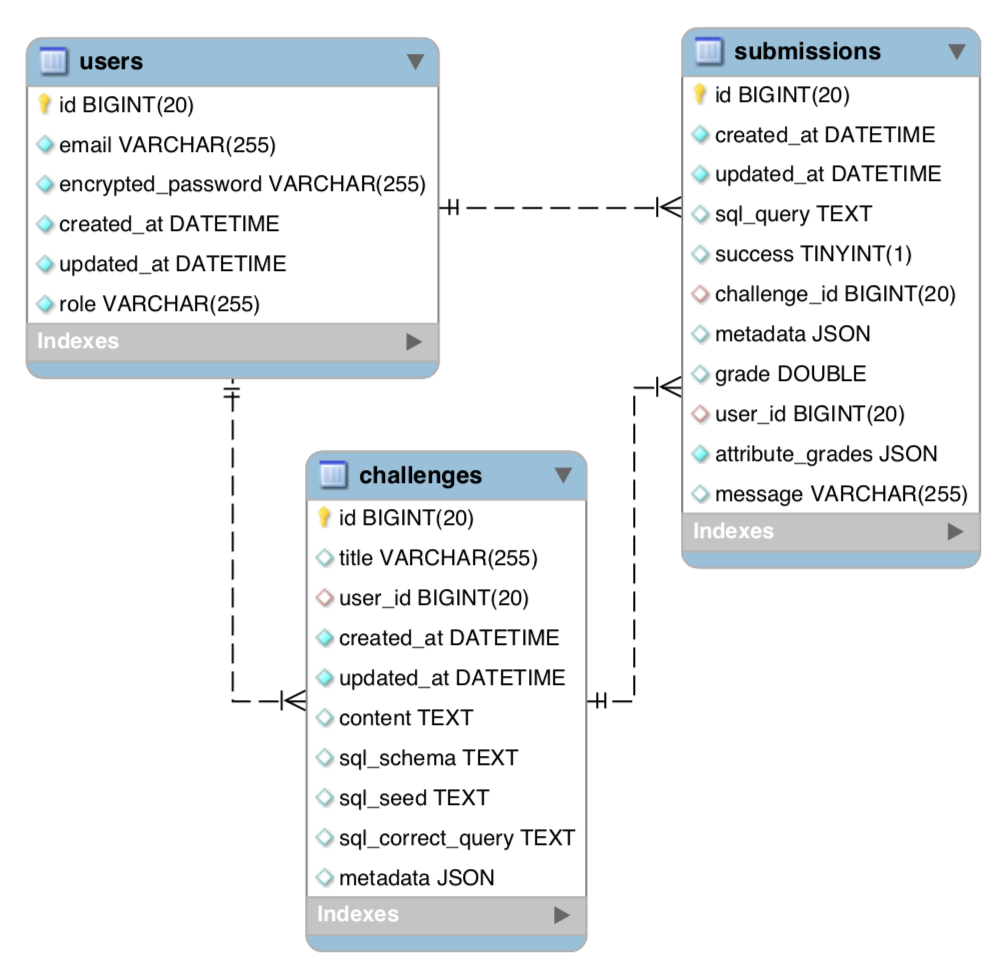
\includegraphics[width=\textwidth/8*6]{Chapters/4-Design/database_schema.png}
    \caption{EER diagram of the web application}
\end{figure}

\subsection{Views}

\begin{figure}[H]
\centering
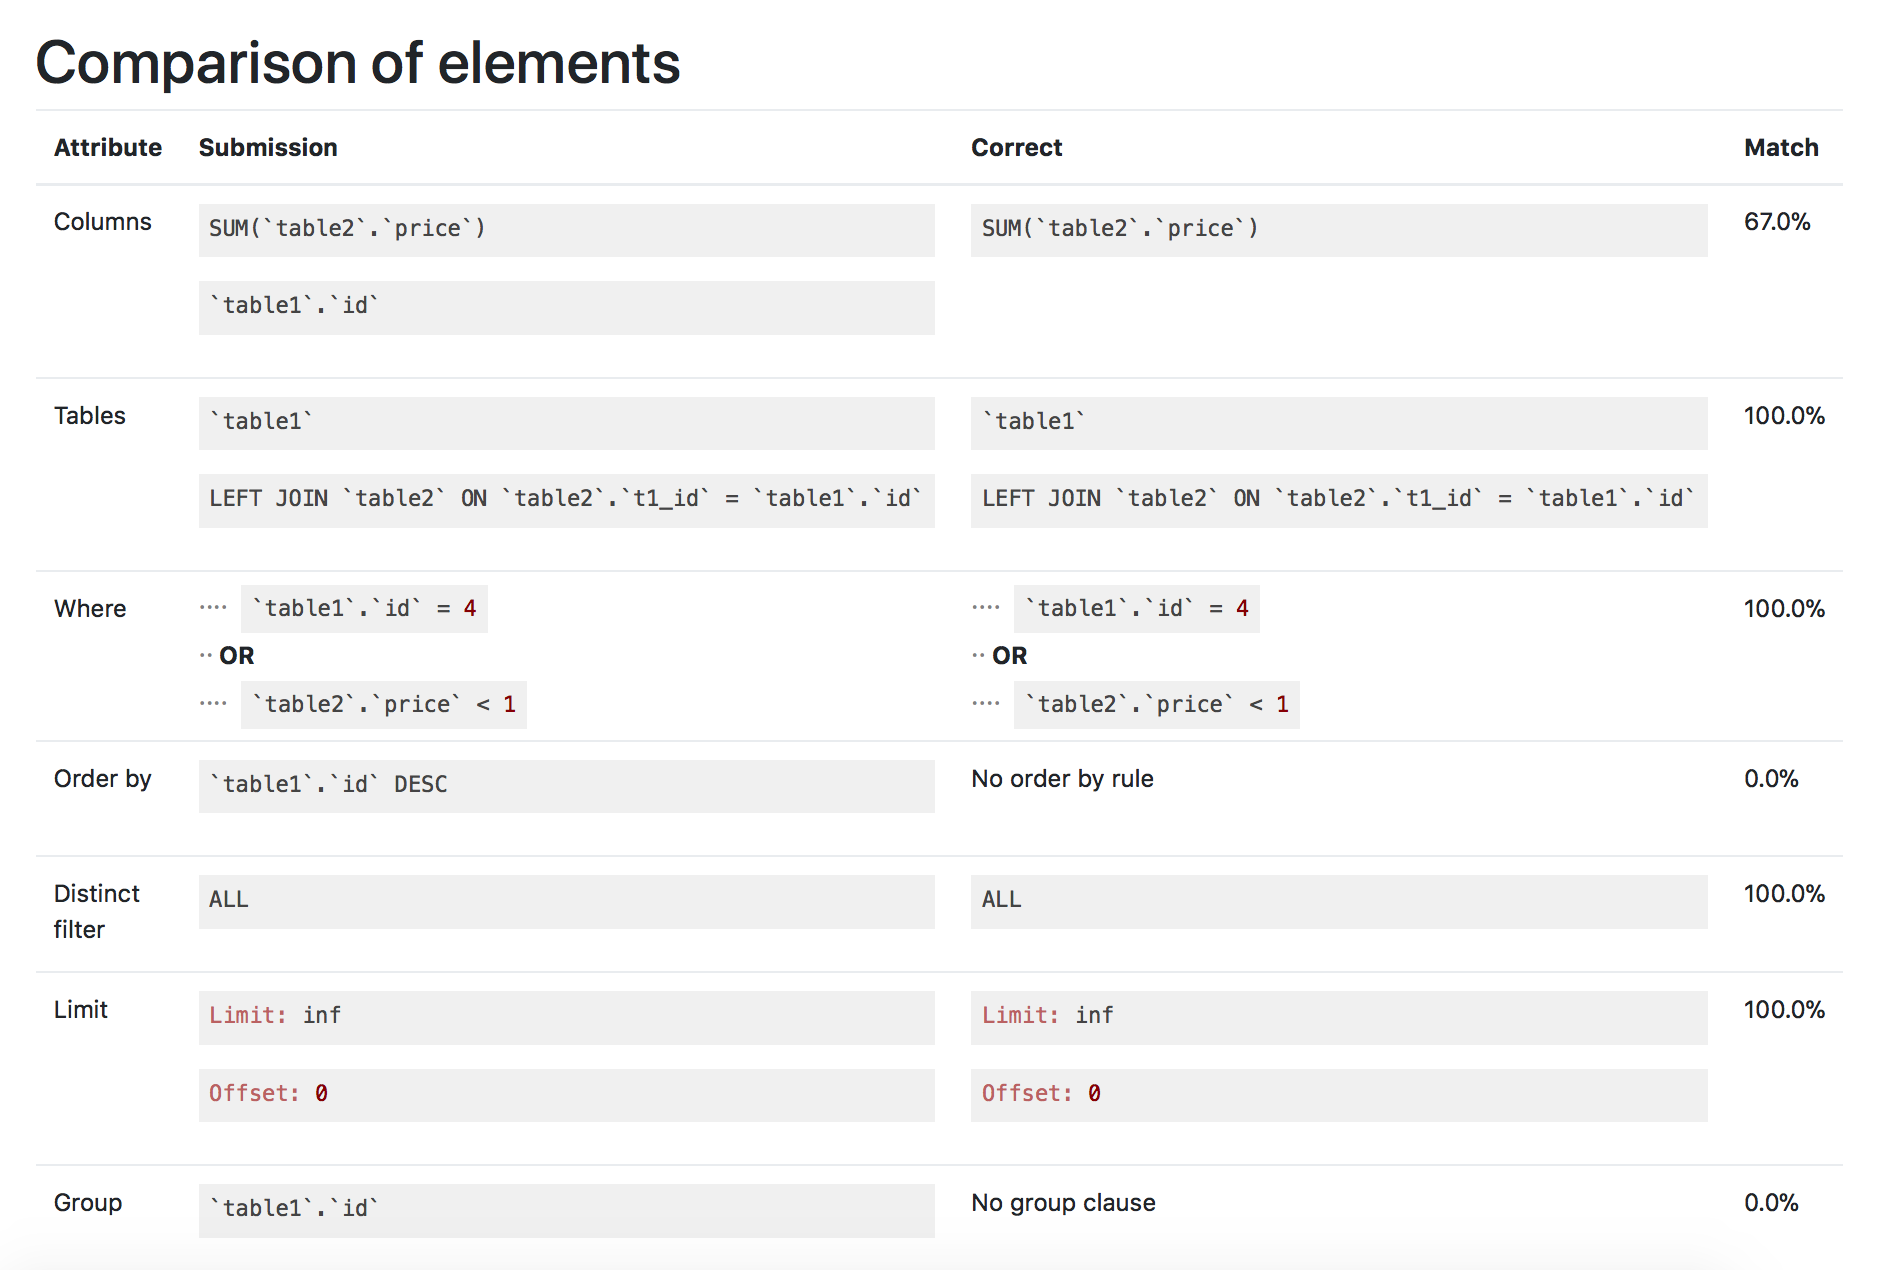
\includegraphics[width=\textwidth]{Chapters/4-Design/components.png}
\caption{Displaying the components of a submission}
\label{fig:design}
\end{figure}


The role of views in a \texttt{MVC} application is to render data \citep{ruby_on_rails}. Most of the application is rendered in \texttt{HTML} (using \mintinline{ruby}{ActionView}) which is displayed in user's browser. The application includes multiple views that serve different purposes: displaying forms, displaying challenge details, etc.

\subsubsection{Design}

The design of the web application will not very advanced. The web application is built using Bootstrap, combined with code highlighting provided by 3rd party libraries (example in figure \ref{fig:design}).


\subsection{Controllers} \label{ch:design:web:controller}

The role of controllers is to \textit{orchestrate} the application. They receive user input (in the form of HTTP requests in the case of Ruby on Rails applications) and returns the correct views which display the correct models \citep{ruby_on_rails_book}. Controllers are implemented as subclasses of \mintinline{ruby}{ActionController::Base} in \texttt{RoR}. This super-class already knows how to handle HTTP requests and return the response to the user. In general, controllers in Ruby on Rails implement the Representational State Transfer (REST) actions. RESTful web services make use of the HTTP methods as following \citep{rodriguez2008restful}:

\begin{tabularx}{\textwidth}{|c|Y|X|X|}
    \hline
    & \textbf{URL} & \textbf{Ruby on Rails action name} & \textbf{Result} \\\hline
    \endhead
    GET & /resource\_name & index & Get all resources \\\hline
    GET & /resource\_name/:id & show & Get resource with given id \\\hline
    GET & /resource\_name/new & new & Get the form for creating a new resource \\\hline
    GET & /resource\_name/:id/edit & edit & Get the form for editing a resource with given id \\\hline
    POST & /resource\_name & create & Create resource \\\hline
    PUT & /resource\_name/:id/ & update & Update a resource with a given id \\\hline
    DELETE & /resource\_name/:id & destroy & Get resource with given id \\\hline
\end{tabularx}

REST Ruby on Rails controllers have in general, in general, the following structure \citep{RoRDocumentation}:
\begin{enumerate}
    \item Receive a web request
    \item Fetch and optionally modify a model
    \item Return a view to the user
\end{enumerate}

The web application built in this project includes the following controllers:
\begin{enumerate}
    \item \textbf{Authentication and user-related controllers}: these controllers handle the basic user management tasks. They are provided by a 3rd-party library called \texttt{devise}.
    \item \mintinline{ruby}{ChallengesController} which defines the REST actions for managing \mintinline{ruby}{Challenge}
    \item \mintinline{ruby}{SubmissionsController} which defines the REST actions for managing \mintinline{ruby}{Submissions}

\end{enumerate}

\section{Example of interaction between user, web application and library and database}

\begin{figure}[H]
    \centering
    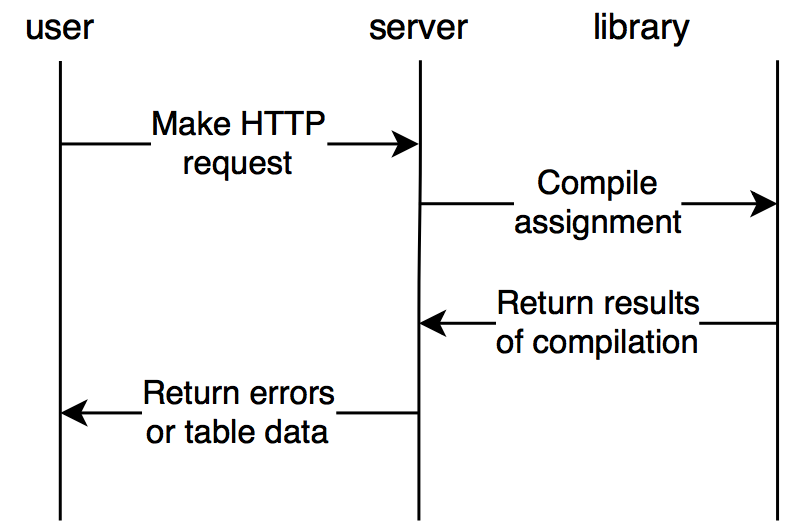
\includegraphics[width=(\linewidth / 2)]{Chapters/4-Design/create_assignment.png}
    \caption{Overview of creating a new assignment}
    \label{fig:create_assignment}
\end{figure}

The user never interacts directly with the library or the database system as all communication from user's perspective is done through the web application.

An example of such an interaction can be seen in figure \ref{fig:create_assignment}. The user makes a POST HTTP requests which is handled by the the Ruby on Rails web application in the \mintinline{ruby}{create} action from \mintinline{ruby}{ChallengesController}. Internally, the controller checks authentication and makes sure the user has the permission to create an assignment. After these checks are made, it then passes on SQL queries received to the library. The library compiles these queries and returns the results or errors. If there are no errors, the tool will create a new \mintinline{ruby}{Challenge} and return a success message to the user as a rendered HTML view. If errors are encountered, they are also rendered to the user as HTML, but no challenge is saved.